%% Viva opening presentation, 10 minutes. Audience: the examiners, who have read the thesis.
%% Framed around the engineer who holds the data: who it is for, what they do with it, and what
%% each method answers for them. Figures copied from the thesis into figures/.
%% Build: pdflatex viva_slides.tex (twice). Timings per slide are in SPEAKER_NOTES.md.
\documentclass[aspectratio=169,11pt]{beamer}
\usetheme{Madrid}
\usecolortheme{seahorse}
\definecolor{ipablue}{HTML}{16548E}
\definecolor{ipared}{HTML}{A23B2E}
\setbeamercolor{structure}{fg=ipablue}
\setbeamercolor{title}{fg=white,bg=ipablue}
\setbeamercolor{frametitle}{fg=white,bg=ipablue}
\setbeamerfont{frametitle}{series=\bfseries}
\setbeamertemplate{navigation symbols}{}
% slim footer: slide number only (the theme's three-box footer clipped)
\setbeamertemplate{footline}{%
  \hfill{\usebeamerfont{page number in head/foot}\color{gray}\insertframenumber}\hspace{1.2em}%
  \vspace{6pt}}
\usepackage{booktabs}
\usepackage{amsmath,amssymb}
\graphicspath{{figures/}}
\newcommand{\good}[1]{\textcolor{ipablue}{#1}}
\newcommand{\bad}[1]{\textcolor{ipared}{#1}}

\title{Information Propagation Methods for Reliability, Reachability and Flow Analysis in
Directed Acyclic Process Networks}
\author{Temitope Ohiani}
\institute{Department of Civil and Environmental Engineering\\University of Strathclyde}
\date{9 October 2026}

\begin{document}

\begin{frame}[plain]\titlepage\end{frame}

%% ------------------------------------------------------------------ 1
\begin{frame}{Who it is for, and the problem}
\begin{columns}[T]
\column{0.52\textwidth}
\textbf{The engineer} responsible for a process system, such as a water treatment works and
its distribution network, asks many questions of it. This thesis addresses three:
\begin{itemize}
  \item Will supply reach each point? \emph{(reliability)}
  \item How much can it deliver, and what limits it? \emph{(capacity)}
  \item How long to restore it, and what is critical? \emph{(schedule)}
\end{itemize}
\medskip
Each has its own method and software, so the \textbf{topology is entered three times} and
kept consistent by hand.
\column{0.45\textwidth}
\textbf{What the engineer actually knows}
\begin{itemize}
  \small
  \item a failure probability from three recorded failures
  \item a nameplate capacity with a tolerance
  \item a duration given as a range, not a number
\end{itemize}
The exact methods in common use take one number per input, so the uncertainty is
\bad{collapsed} before the analysis runs.

\medskip
\small And the system model is often sensitive: it should \textbf{stay on the engineer's
machine}.
\end{columns}
\end{frame}

%% ------------------------------------------------------------------ 2
\begin{frame}{One model, three interpretations}
\begin{columns}[c]
\column{0.40\textwidth}
\centering
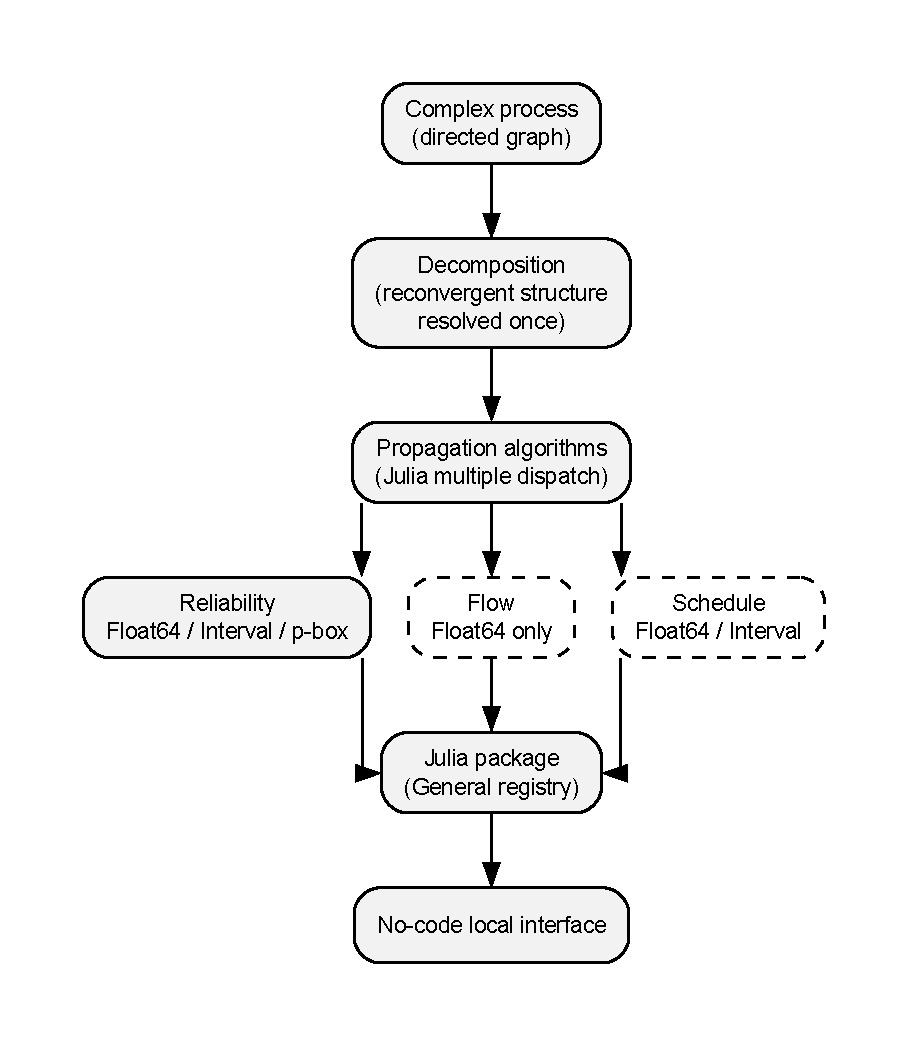
\includegraphics[width=\linewidth,height=0.72\textheight,keepaspectratio]{fig01_framework_overview.pdf}
\column{0.58\textwidth}
\small
A system is a \textbf{DAG}: components are nodes, dependencies are edges. One \textbf{graph
object} is read by three toolkits; only the meaning of the value on a component changes, a
failure probability, a throughput limit or a duration. A further analysis would read the same
object.

\medskip
\textbf{Research questions}
\begin{enumerate}
  \item Can one DAG model serve all three analyses, topology entered once?
  \item Can reconvergence be identified once and reused?
  \item Exact reliability under intervals and p-boxes: what is guaranteed, at what cost?
  \item Which critical-path quantities stay exact under interval durations?
  \item Can it reach an engineer who does not program, with the model kept on their machine?
\end{enumerate}
\end{columns}
\end{frame}

%% ------------------------------------------------------------------ 3
\begin{frame}{What the engineer does with it}
\centering
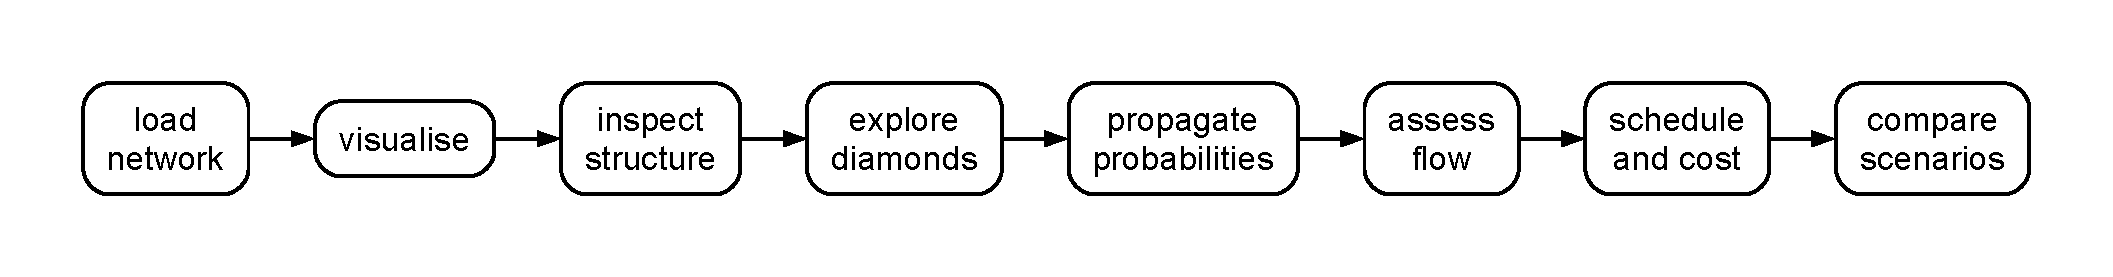
\includegraphics[width=0.92\linewidth]{fig00_pipeline.pdf}
\vspace{2pt}
\begin{columns}[c]
\column{0.50\textwidth}
\small
\begin{itemize}
  \item Uploads the files they already have: an edge list and one JSON file per analysis.
  No code.
  \item Every result keeps the form its inputs were given in, an interval stays an interval,
  and names its method: \emph{exact}, \emph{sound} or \emph{conservative enclosure}.
  \item Runs on their own machine: a browser interface over a loopback server.
  \item The same methods are a registered Julia package,
  \texttt{InformationPropagationAnalysis.jl}, for scripted use.
\end{itemize}
\column{0.47\textwidth}
\centering
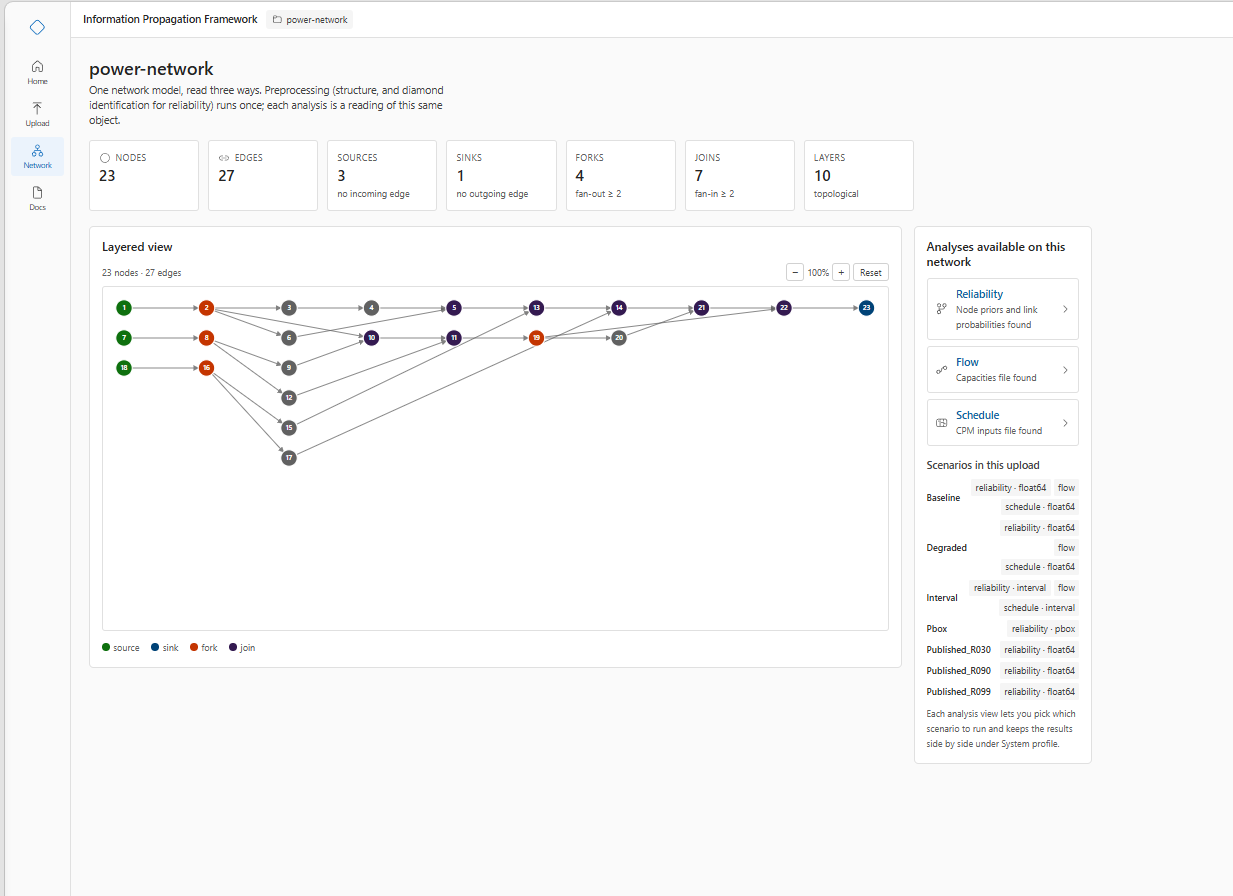
\includegraphics[width=\linewidth,height=0.48\textheight,keepaspectratio]{fe_network.png}\\
\scriptsize the network page after upload
\end{columns}
\end{frame}

%% ------------------------------------------------------------------ 4
\begin{frame}{Will supply reach each point? Redundancy is what makes it hard}
\begin{columns}[c]
\column{0.30\textwidth}
\centering
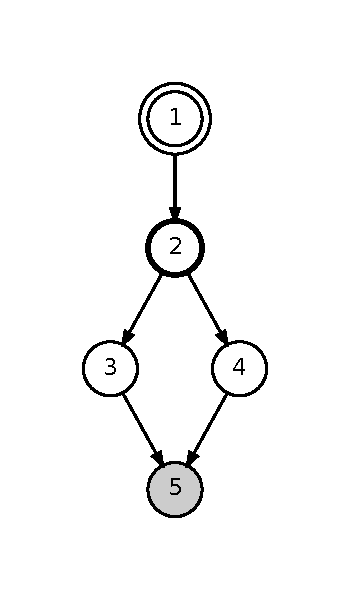
\includegraphics[width=0.8\linewidth,height=0.52\textheight,keepaspectratio]{fig01_simple_diamond.pdf}\\
\footnotesize every component $0.9$
\column{0.66\textwidth}
\small
Redundant routes split and rejoin, sharing what is upstream. Treating them as independent
\bad{overstates} reliability: $b(5) = 0.749$ against the exact $0.675$.

\medskip
Conditioning on the fork's reachability repairs it exactly:
\[
b(5) = 0.9\,\bigl[\,0.81 \times \bigl(1-(1-0.729)^2\bigr) + 0.19 \times 0\,\bigr] = 0.675462
\]
Two sub-problems replace $2^{9}$ states of the uncertain components.

\medskip
The \textbf{Network Decomposition Module} finds every such \emph{diamond} once, with its
\textbf{conditioning set}, proved complete, deterministic and terminating.
\end{columns}
\end{frame}

%% ------------------------------------------------------------------ 5
\begin{frame}{How sure can the engineer be? Reliability with uncertain inputs}
\begin{columns}[c]
\column{0.5\textwidth}
\small
One pass over the network, conditioning at each join. The answer comes back in the form
the inputs were given:
\begin{itemize}
  \item \textbf{numbers}: the exact reliability of every node;
  \item \textbf{intervals}: the exact range, because reliability is monotone in each input;
  \item \textbf{p-boxes}: sound bounds on its distribution.
\end{itemize}
Agrees with a decision-diagram oracle to $1.1\times10^{-16}$ on 129 graphs.

\medskip
\textbf{Cost}: exponential in the largest conditioning set, the same width a decision diagram
pays. The gain is the uncertainty carried through, not speed.
\column{0.48\textwidth}
\centering
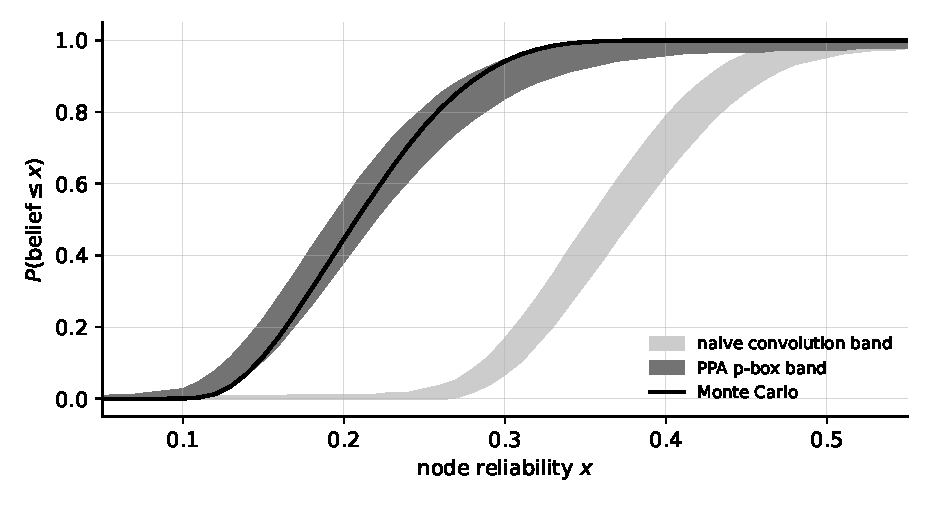
\includegraphics[width=\linewidth,height=0.6\textheight,keepaspectratio]{fig08_hero_cdf.pdf}\\
\footnotesize the p-box band brackets the Monte Carlo distribution
\end{columns}
\end{frame}

%% ------------------------------------------------------------------ 6
\begin{frame}{How much can it deliver, and what limits it?}
\begin{columns}[c]
\column{0.46\textwidth}
\small
\textbf{Capacity} (point-valued)
\begin{itemize}
  \item Throughput, every minimum cut, saturated edges, single points of failure, how far an
  edge can degrade or must be upgraded.
  \item All minimum cuts from one solve: the closed subsets of the free zone (Picard and
  Queyranne), at most $2^{|\mathcal{F}|}$.
  \item Two designs deliver the same 37 units; one has 4 minimum cuts, the other 1. Where the
  network binds differs, and so does what to reinforce.
\end{itemize}
\column{0.52\textwidth}
\centering
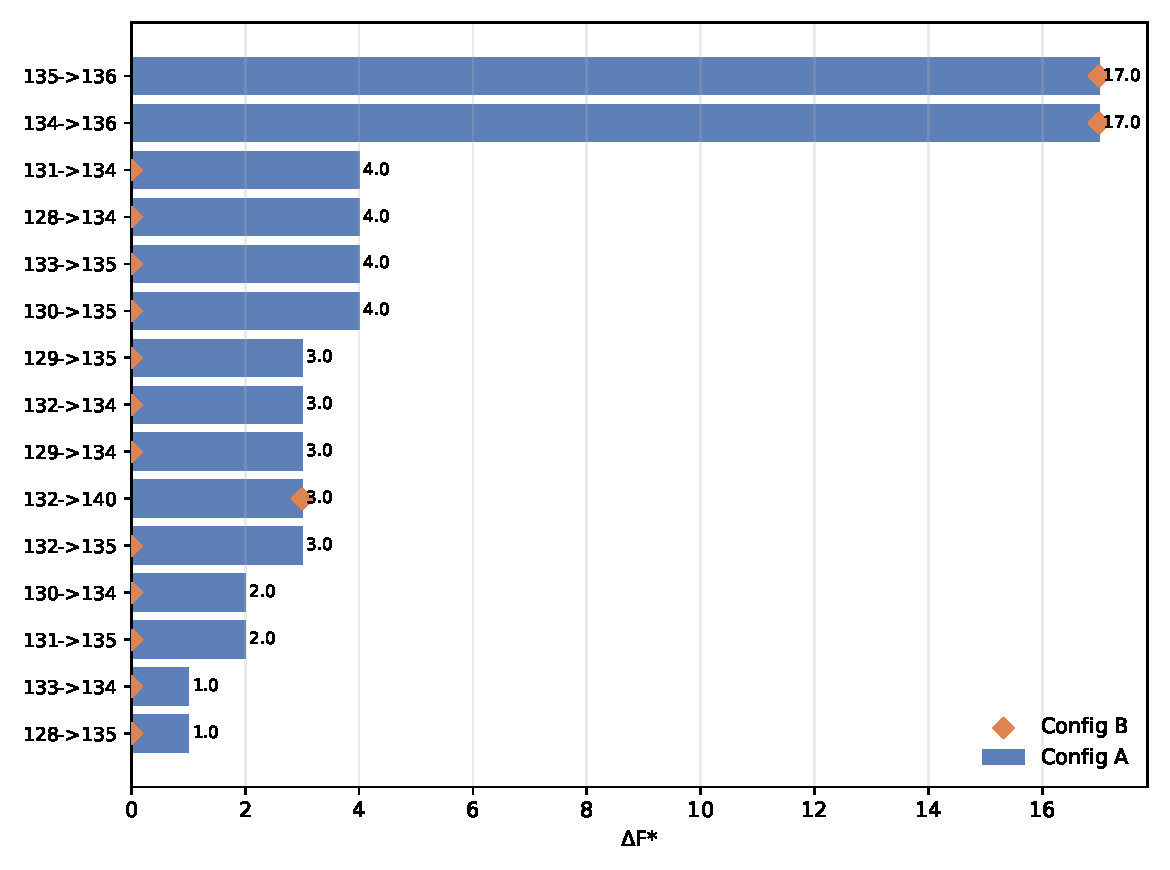
\includegraphics[width=\linewidth,height=0.62\textheight,keepaspectratio]{critical_bars_config_ab.pdf}\\
\footnotesize loss in throughput when one edge fails: design A (bars) has 15 edges that
matter, design B (markers) has 3
\end{columns}
\end{frame}

\begin{frame}{How long to restore it, and what is critical?}
\begin{columns}[c]
\column{0.50\textwidth}
\small
\textbf{Schedule}
\begin{itemize}
  \item Critical path generalised to a family of operator pairs; with interval durations, the
  completion time is exact from two runs.
  \item Which activities are critical \emph{whatever} the durations turn out to be
  (\emph{necessarily}), or only for some (\emph{possibly})? In general this means trying every
  duration at its low or high end: $2^k$ runs, and NP-hard. The \textbf{domination split} varies
  only the durations that can route around each activity.
  \item 30-activity PSPLIB benchmark: 50,524 runs instead of $2^{30}$ ($\approx$1.1 billion).
  It found 3 activities critical whatever happens, which the fast conservative method could
  not confirm, and cleared 7 that it had flagged.
\end{itemize}
\column{0.47\textwidth}
\centering
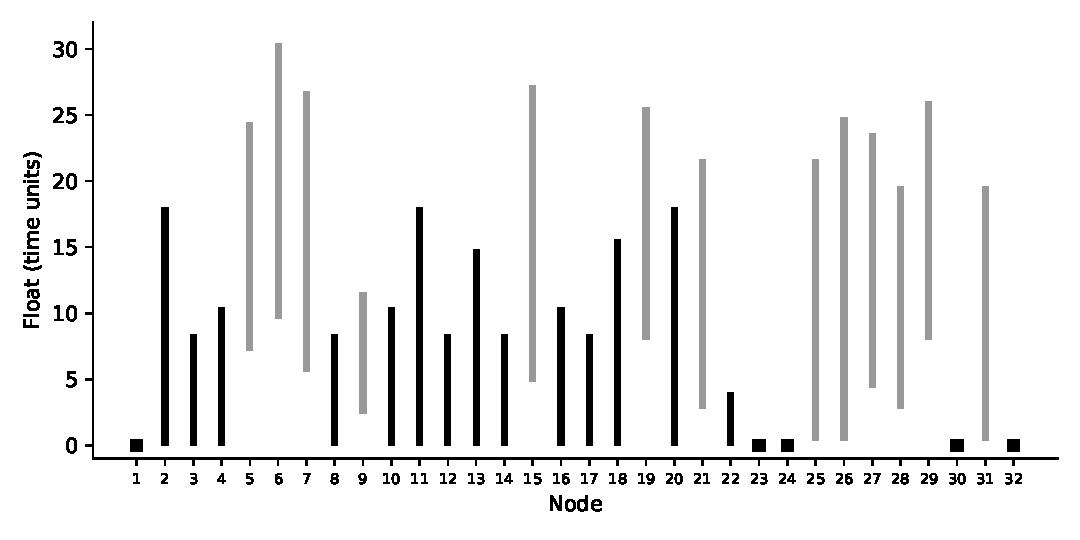
\includegraphics[width=\linewidth,height=0.62\textheight,keepaspectratio]{fig04_floats.pdf}\\
\footnotesize exact float range of each activity, durations $\pm20\%$: points at zero are
critical in every case
\end{columns}
\end{frame}

%% ------------------------------------------------------------------ 7
\begin{frame}{One water network, three questions: EPANET Net3}
\begin{columns}[T]
\column{0.5\textwidth}
\small
97 nodes, 119 edges, oriented by its own hydraulic simulation; converted once.
\begin{itemize}
  \item \textbf{Reliability}: worst-served junction $0.81$; $[0.35, 0.99]$ under $\pm5\%$.
  \item \textbf{Capacity}: whole demand met, \good{680.1 L/s}; river pump out,
  \good{43.3 L/s} (6.4\%).
  \item \textbf{Schedule}: 74 days along 28 activities; $[59, 89]$ days under intervals.
\end{itemize}
\column{0.47\textwidth}
\small
For the engineer: the \textbf{river pump} (95--97, \bad{red}) is in every degraded minimum cut
\emph{and} on the restoration critical chain. Reinstating it is the step both analyses point
to, which neither shows alone.

\medskip
\scriptsize\textit{Corrected since submission: the super-sink edges were missing from the flow
graph. Errata sheet provided.}
\end{columns}
\vspace{4pt}
\centering
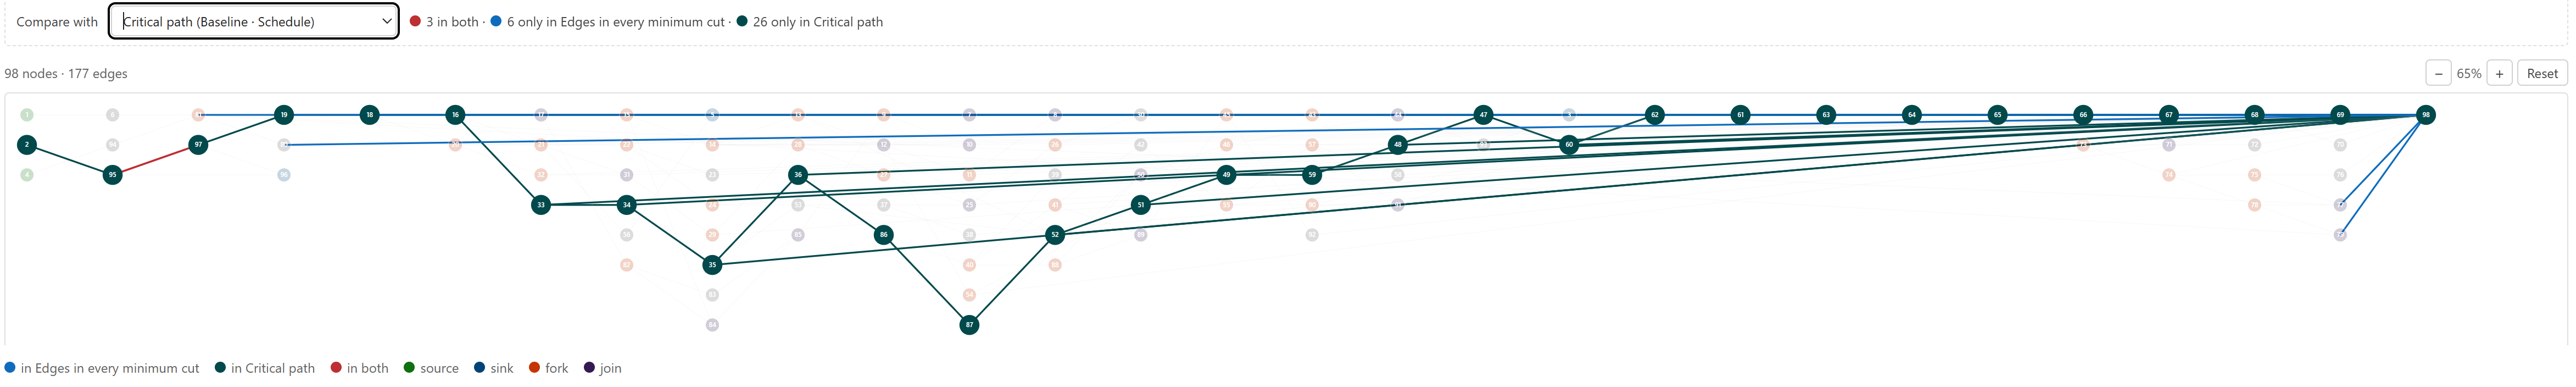
\includegraphics[width=\linewidth,height=0.36\textheight,keepaspectratio]{net3_overlay_crop.png}\\
\scriptsize Degraded minimum cut (blue) against the baseline critical path (dark): 95, 97 and
the super-sink in both.
\end{frame}

%% ------------------------------------------------------------------ 8
\begin{frame}{Answers, contributions and limits}
\begin{columns}[T]
\column{0.52\textwidth}
\small
\textbf{Answers}
\begin{enumerate}
  \item Yes, on the model's four assumptions.
  \item Yes, for the probabilistic interpretation.
  \item Exact for numbers and intervals, sound for p-boxes; cost set by conditioning width.
  \item Completion time in two runs; floats exact at a cost set by bypass width.
  \item Yes: a registered package and a local no-code interface.
\end{enumerate}
\column{0.45\textwidth}
\small
\textbf{Limits, stated in the thesis}
\begin{itemize}
  \item Practical to conditioning width about 18 (about 50 nodes, moderate reconvergence); p-boxes on small networks.
  \item Capacity is point-valued.
  \item Acyclicity is a property of one operating snapshot.
  \item The interface is demonstrated, not yet studied with engineers in use.
\end{itemize}
\smallskip
\footnotesize\textbf{Next}: a depth-limited hybrid for larger networks; interval capacities; cyclic
networks; a study with engineers in use.\\[2pt]
\textbf{Demo}: \texttt{information-propagation-framework.dev}
\end{columns}
\end{frame}

\begin{frame}[plain]
\centering\vfill\Large Thank you\\[8pt]
\normalsize Questions welcome\vfill
\end{frame}

%% ================================================================== backup
%% Not presented. Kept after the close so a likely question can be answered from a prepared
%% slide.
\appendix
\begin{frame}{Backup: how does an engineer get their network in?}
\small
\begin{itemize}
  \item \textbf{Structure}: an edge list or an adjacency matrix, the form any DAG description
  reduces to. The parser detects which, validates acyclicity and builds the graph object once.
  \item \textbf{Inputs}: one JSON file per analysis, which declares its value form (number,
  interval or p-box), so the same network carries probabilities, capacities and durations side
  by side.
  \item \textbf{From a domain model}: Net3 came from its EPANET \texttt{.inp} file by a script
  that orients each pipe by its simulated flow and derives the three input files from pipe
  diameters, pump curves and published break rates (in the thesis-data repository).
  \item \textbf{Limit, stated in the thesis}: the package itself does not read domain formats
  such as EPANET or a GIS export; that conversion is a script per source.
\end{itemize}
\end{frame}

\begin{frame}{Backup: what would you do next?}
\small
Each item follows from a limitation stated in the thesis (Chapter 11).
\begin{itemize}
  \item \textbf{Scale}: a depth-limited hybrid, exact to a stated depth and bounded beyond it,
  for networks past about fifty nodes of moderate reconvergence.
  \item \textbf{Theory}: a soundness proof for the tighter p-box recombination operator,
  validated sound on every configuration tested but not proved.
  \item \textbf{Schedule}: gate the domination split by its own bypass-set cost in place of a
  fixed threshold; that threshold sent Net3 to the conservative enclosure.
  \item \textbf{Capacity}: interval and p-box capacities, direct for the flow value by
  monotonicity, open for the cut structure.
  \item \textbf{Model}: cyclic networks by strongly connected components or unrolling, and an
  orientation per operating state (Net3's degraded case).
  \item \textbf{Use}: a study of the interface with engineers who do not program.
\end{itemize}
\end{frame}

\begin{frame}{Backup: what changed since submission?}
\small
\textbf{Chapter 6.} ``Exactly $2^{|\mathcal{F}|}$ minimum cuts'' becomes ``at most'':
$S^\star\cup R$ is a minimum cut iff $R\subseteq\mathcal{F}$ is closed under residual
reachability (Picard and Queyranne, 1980). Implementation corrected; every Chapter 6 result
re-run and unchanged (Configuration A: 4 cuts; B: 1).

\medskip
\textbf{Chapter 10.} The flow run used the edge list without the super-sink and its 58 demand
edges, and reported 1,837.9 L/s, above the total demand of 680.1. The algorithms were correct;
the server in the interface layer ignored the 58 entries without reporting them.
\begin{center}
\begin{tabular}{@{}lll@{}}
\toprule
& Submitted & Corrected \\
\midrule
Baseline throughput & 1,837.9 L/s & 680.1 L/s (all demand) \\
Baseline minimum cut & 4 supply edges & the 58 demand edges \\
Degraded throughput & 954.6 L/s & 43.3 L/s (6.4\%) \\
Degraded minimum cuts & same 4 & 24; river pump in every one \\
Overlay with critical path & ``no node in common'' & river pump on both \\
\bottomrule
\end{tabular}
\end{center}
Checked against an independent Edmonds--Karp computation. Reliability and schedule unchanged.
\end{frame}

\begin{frame}{Backup: why does Net3 deliver so little with the river pump out?}
\small
\begin{itemize}
  \item With the river pump out, the sources are the lake pump and one discharging tank.
  \item In the snapshot orientation they reach only six junctions (7, 8 and 77--81), which are
  fully served; the other 52 receive less than their demand.
  \item The derated trunk main does not bind: its only feed is the river pump.
  \item Physically, the lake pump could push water through pipes that ran the other way at the
  snapshot. The oriented model cannot represent that. A degraded state needs an orientation of
  its own.
\end{itemize}
\end{frame}

\begin{frame}{Backup: how can interval floats be exact when the problem is NP-hard?}
\begin{columns}[c]
\column{0.45\textwidth}
\centering
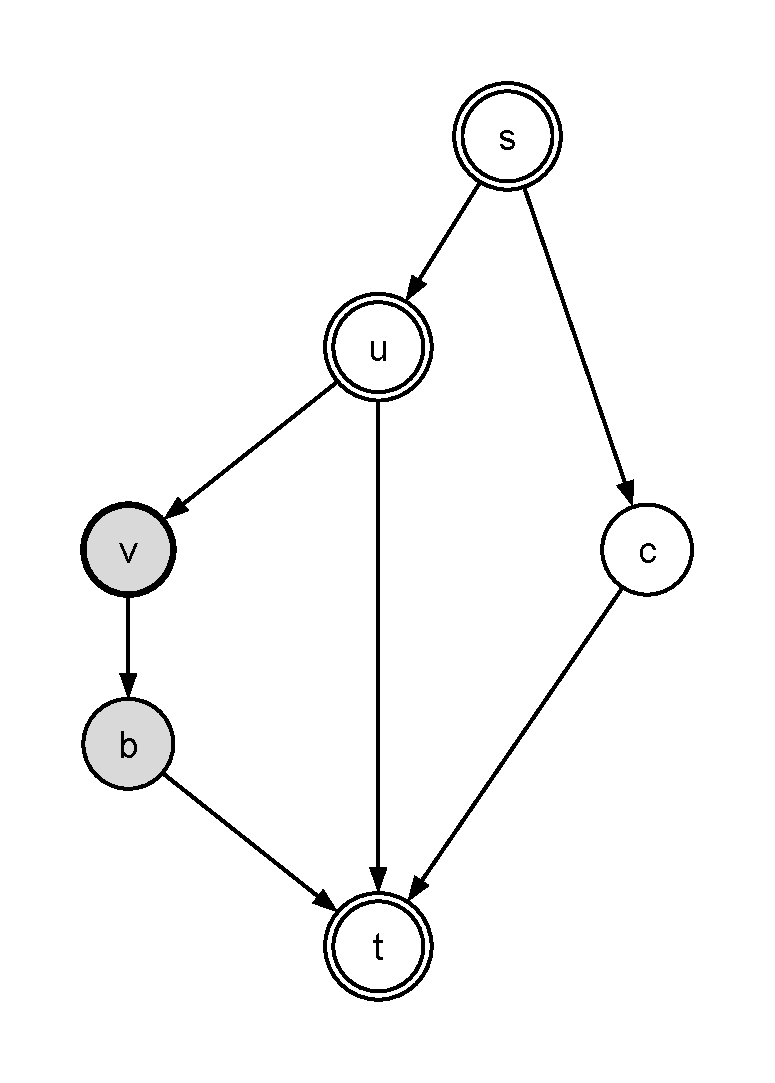
\includegraphics[width=\linewidth,height=0.65\textheight,keepaspectratio]{fig02_bypass.pdf}
\column{0.52\textwidth}
\small
Relative to node $v$: \emph{dominated} durations (every route through them passes $v$) are
fixed at one bound, \emph{incomparable} ones at the other, and only the \emph{bypass set}
$H_v$, which shares routes with $v$ and can route around it, is enumerated.

\medskip
The exact floats then cost $2\sum_v 2^{|H_v|}$ propagations in all, against $2^k$ for
$k$ interval durations.
\end{columns}
\end{frame}

\begin{frame}{Backup: how are p-boxes combined at a diamond?}
\small
\textbf{Chain and union steps}: the quantities combined are independent for the same
structural reason the point computation is exact, so p-box arithmetic under independence
applies (Williamson and Downs).

\medskip
\textbf{The conditioning step} is the convex combination
\[ W\cdot A + (1-W)\cdot B \]
where $A$, $B$ depend on the same upstream reliabilities, and $W$, $1-W$ are one variable.
Convolving the terms as if independent is \bad{unsound}: probability mass leaves $[0,1]$, by
up to $0.34$ on the benchmark grid.

\medskip
\textbf{The operator}: at each discretisation level of $W$, weight the branches by $w$ and
$1-w$, combine them under a dependence bound, mix across levels, and envelope the results built
on $W$'s two bounding functions. Taking one conditioning node at a time reproduces the mixture
over all $2^{|C|}$ states. The output is clipped to $[0,1]$, with a guard that raises an error
if the excursion is more than round-off.
\end{frame}

\begin{frame}{Backup: is the p-box result sound?}
\begin{columns}[T]
\column{0.52\textwidth}
\small
\textbf{Two dependence bounds} for the branches
\begin{itemize}
  \item \textbf{Fr\'echet--Hoeffding}: sound for \emph{any} dependence by a classical theorem;
  can be wide, near vacuous on hard cases.
  \item \textbf{Positive dependence} (default): $A$ and $B$ both rise with the shared upstream
  reliabilities. Tighter; no violation in 50 configurations against Monte Carlo.
  \bad{Not proved}: no theorem covers positive but otherwise unknown dependence, and the
  ordering-of-dependence route fails (the distributions cross).
\end{itemize}
Fr\'echet is used wherever a claim must rest on proof alone.
\column{0.45\textwidth}
\small
\textbf{What it buys}
\begin{itemize}
  \item Band width $0.18$ under high reliability and weak reconvergence, $0.70$ under deep
  reconvergence with broad uncertainty; no violations in the sweep.
  \item For a requirement $x^\ast = 0.95$: $P(b(v)\le x^\ast)$ certified to a band of
  $0.02$--$0.12$ from one propagation.
  \item Simulation would need 267 to 9,604 samples, and gives an estimate, not a bound.
\end{itemize}
\end{columns}
\end{frame}

\begin{frame}{Backup: is it faster than a decision diagram?}
\centering
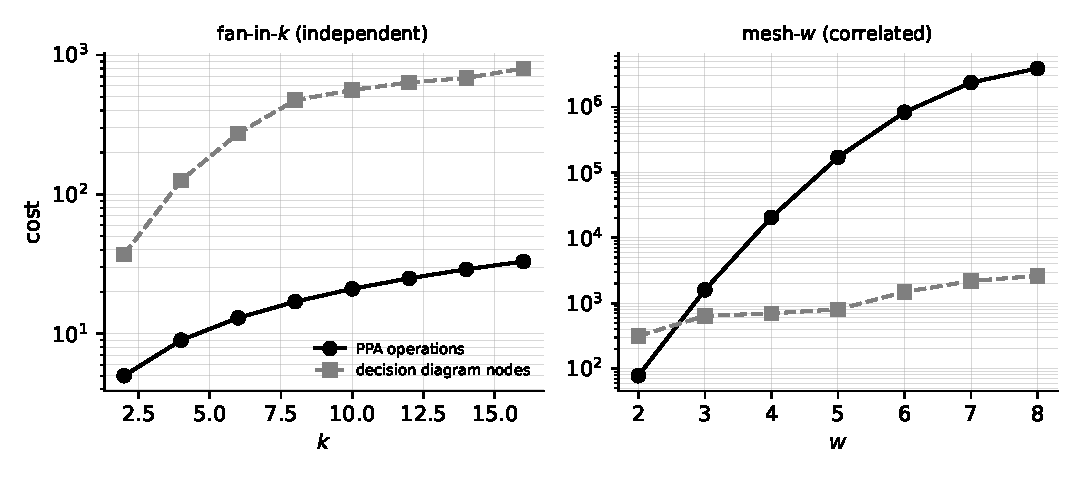
\includegraphics[width=0.85\linewidth,height=0.7\textheight,keepaspectratio]{fig07_crossover.pdf}\\
\small Sub-problem count against sifted BDD node count on the two adversarial families
(fan-in-$k$, mesh-$w$).
\end{frame}

\end{document}
